\section{Examples of convolution filters and performance}
In this section, we will give a brief description how convolution operations are used for image processing.
One useful description can be found in the following link:

\href{http://aishack.in/tutorials/image-convolution-examples/}{http://aishack.in/tutorials/image-convolution-examples/}

Convolutions is a technique for general signal processing. People studying electrical/electronics will tell you the near-infinite sleepless nights these convolutions have given them. Entire books have been written on this topic. And the questions and theorems that need to be proved are insurmountable. But for computer vision, we'll just deal with some simple things.

A convolution lets you do a very wide variety of things, like calculating derivatives, detecting edges, apply ing blurs, etc. And all of this is done with a "convolution kernel".

\subsection{Calculation with convolutions}
The most direct way to compute a convolution would be to use multiple for loops. But that causes a lot of repeated calculations. And as the size of the image and kernel increases, the time to compute the convolution increases quite drastically.

Techniques haves been developed to calculate convolutions rapidly. One such technique is using the Discrete Fourier Transform. It converts the entire convolution operation into a simple multiplication. Fortunately, you don't need to know the math to do this in OpenCV. It automatically decides whether to do it in frequency domain (after the DFT) or not.

\subsection{Image convolution examples}
A convolution is very useful for signal processing in general. There is a lot of complex mathematical theory available for convolutions. For digital image processing, you don't have to understand all of that. You can use a simple matrix as an image convolution kernel and do some interesting things!


\subsection{Line detection by 1D Laplacian}
With image convolutions, you can easily detect lines. Figure \ref{line:detect1} represents the  four convolutions to detect horizontal, vertical and lines at 45 and 135 degrees:
\begin{figure}[!ht]
	\centering
	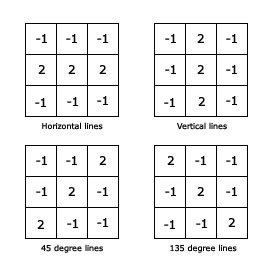
\includegraphics[width=.4\textwidth]{6DL/figures/line}
	\caption{Four convolutions to detect horizontal, vertical and lines at degrees 0,90,45,135.}
	\label{line:detect1}
\end{figure}
Figure \ref{line:detect2}, \ref{line:detect4}, \ref{line:detect6} and \ref{line:detect8} plot the  0,90,45,135 lines detection that I got on an image.
%I looked for horizontal lines on the house image. The result I got for this image convolution was: 
\begin{figure}[!ht]
	\centering
	\subfigure[image]{
		%\label{fig:subfig:a} %% label for first subfigure
		
\includegraphics[width=1.3in]{6DL/figures/xu-0401/image.png}
	}
	\subfigure[filter]{
		%\label{fig:subfig:b} %% label for second subfigure
		\includegraphics[width=1.0in]{6DL/figures/xu-0401/line-detection-0-k.png}
	}
	\subfigure[result]{
		%\label{fig:subfig:b} %% label for second subfigure
		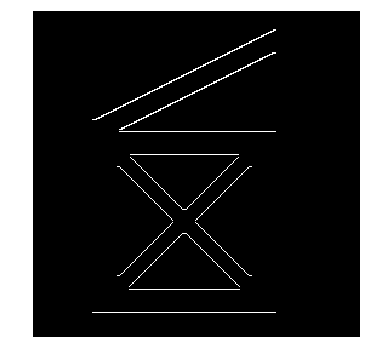
\includegraphics[width=1.3in]{6DL/figures/xu-0401/line-detection-0.png}
	} 
	\caption{~~A horizontal line detection done with convolutions.}
	\label{line:detect2}
	%\label{fig:subfig} %% label for entire figure
\end{figure}

%\begin{figure}[H]
%	\centering
%	\subfigure[image]{
%		%\label{fig:subfig:a} %% label for first subfigure
%		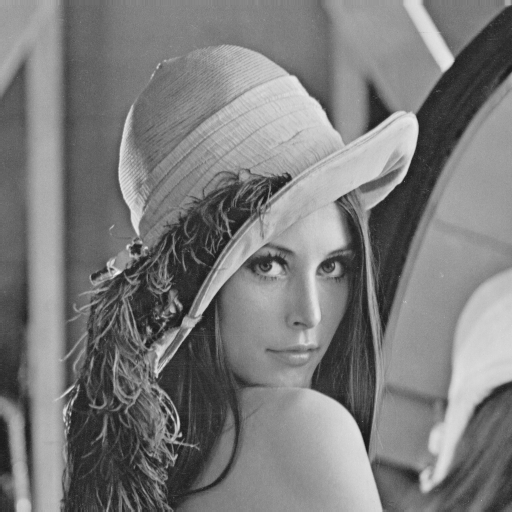
\includegraphics[width=1.3in]{6DL/figures/xu-0401/lena.png}
%	}
%	%\subfigure[filter]{
%		%\label{fig:subfig:b} %% label for second subfigure
%	%	\includegraphics[width=1in]{xu-0401/line-detection-0-k.png}
%	%}
%	\subfigure[result]{
%		%\label{fig:subfig:b} %% label for second subfigure
%		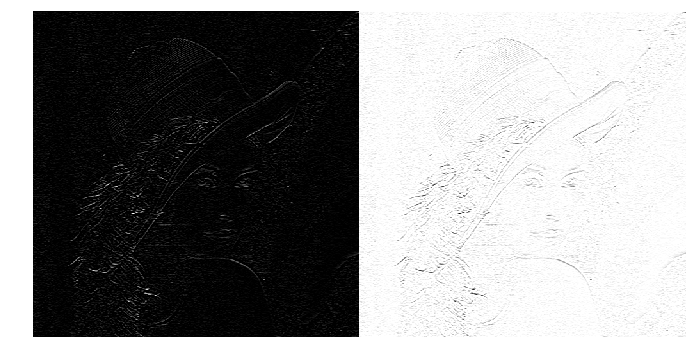
\includegraphics[width=2.6in]{6DL/figures/xu-0401/lena_line_0.png}
%	}
%	\caption{~~A horizontal line detection for Lena.}
%	\label{line:detect3}
%	%\label{fig:subfig} %% label for entire figure
%\end{figure}
In Figure \ref{line:detect4}, the black background is the original result, the white background is obtained by subtracting the original result from 255, the same below.
\begin{figure}[H]
	\centering
	\subfigure[image]{
		%\label{fig:subfig:a} %% label for first subfigure
		
\includegraphics[width=1.3in]{6DL/figures/xu-0401/image.png}
	}
	\subfigure[filter]{
		%\label{fig:subfig:b} %% label for second subfigure
		\includegraphics[width=1.0in]{6DL/figures/xu-0401/line-detection-90-k.png}
	}
	\subfigure[result]{
		%\label{fig:subfig:b} %% label for second subfigure
		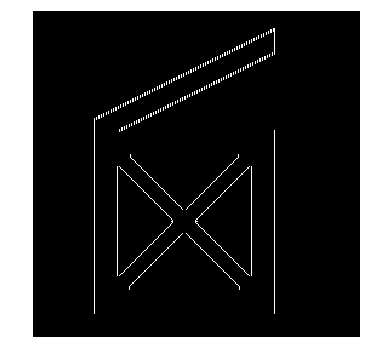
\includegraphics[width=1.3in]{6DL/figures/xu-0401/line-detection-90.png}
	}
	\caption{~~A vertical line detection done with convolutions.}
	\label{line:detect4}
	%\label{fig:subfig} %% label for entire figure
\end{figure}

%\begin{figure}[H]
%	\centering
%	\subfigure[image]{
%		%\label{fig:subfig:a} %% label for first subfigure
%		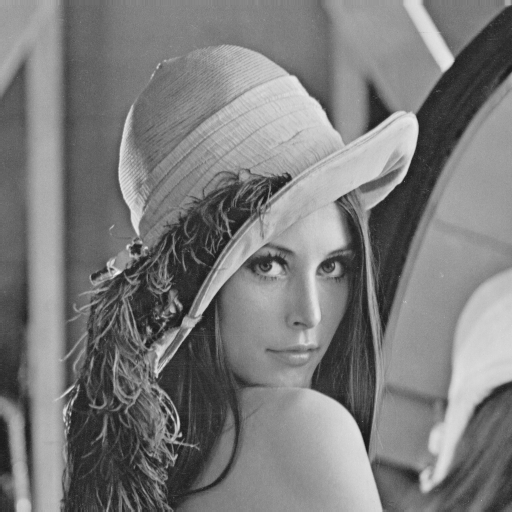
\includegraphics[width=1.3in]{6DL/figures/xu-0401/lena.png}
%	}
%	%\subfigure[filter]{
%		%\label{fig:subfig:b} %% label for second subfigure
%	%	\includegraphics[width=1.0in]{xu-0401/line-detection-90-k.png}
%	%}
%	\subfigure[result]{
%		%\label{fig:subfig:b} %% label for second subfigure
%		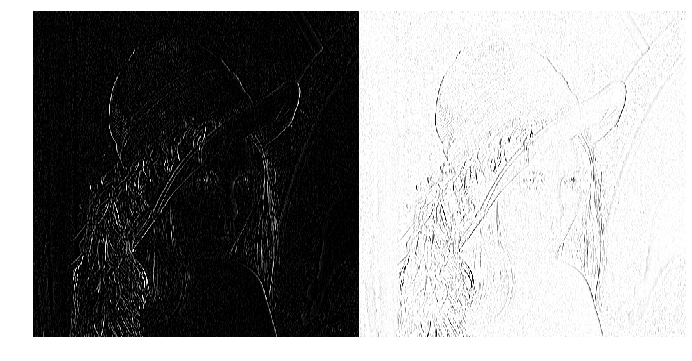
\includegraphics[width=2.6in]{6DL/figures/xu-0401/lena_line_90.png}
%	} 
%	\caption{~~A vertical line detection for Lena.}
%	\label{line:detect5}
%	%\label{fig:subfig} %% label for entire figure
%\end{figure}


\begin{figure}[H]
	\centering
	\subfigure[image]{
		%\label{fig:subfig:a} %% label for first subfigure
		
\includegraphics[width=1.3in]{6DL/figures/xu-0401/image.png}
	}
	\subfigure[filter]{
		%\label{fig:subfig:b} %% label for second subfigure
		\includegraphics[width=1.0in]{6DL/figures/xu-0401/line-detection-45-k.png}
	}
	\subfigure[result]{
		%\label{fig:subfig:b} %% label for second subfigure
		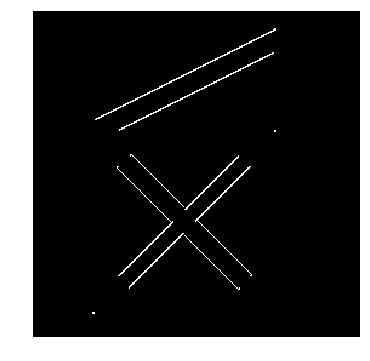
\includegraphics[width=1.3in]{6DL/figures/xu-0401/line-detection-45.png}
	}
	%\label{fig:subfig} %% label for entire figure
	\caption{~~A 45 degree line detection done with convolutions.}
	\label{line:detect6}
\end{figure}

%\begin{figure}[H]
%	\centering
%	\subfigure[image]{
%		%\label{fig:subfig:a} %% label for first subfigure
%		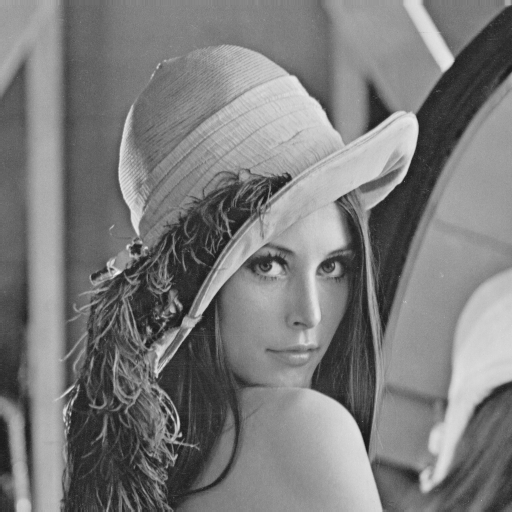
\includegraphics[width=1.3in]{6DL/figures/xu-0401/lena.png}
%	}
%	%\subfigure[filter]{
%		%\label{fig:subfig:b} %% label for second subfigure
%	%	\includegraphics[width=1.0in]{xu-0401/line-detection-45-k.png}
%	%}
%	\subfigure[result]{
%		%\label{fig:subfig:b} %% label for second subfigure
%		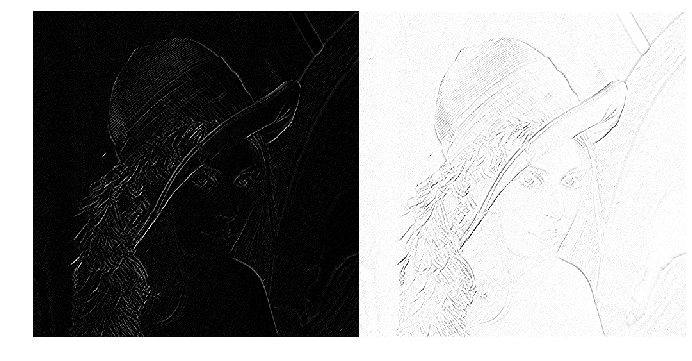
\includegraphics[width=2.6in]{6DL/figures/xu-0401/lena_line_45.png}
%	}
%	\caption{~~A 45 degree line detection done with convolutions} 
%	\label{line:detect7}
%	%\label{fig:subfig} %% label for entire figure
%	
%\end{figure}

\begin{figure}[H]
	\centering
	\subfigure[image]{
		%\label{fig:subfig:a} %% label for first subfigure
		
\includegraphics[width=1.3in]{6DL/figures/xu-0401/image.png}
	}
	\subfigure[filter]{
		%\label{fig:subfig:b} %% label for second subfigure
		\includegraphics[width=1.0in]{6DL/figures/xu-0401/line-detection-135-k.png}
	}
	\subfigure[result]{
		%\label{fig:subfig:b} %% label for second subfigure
		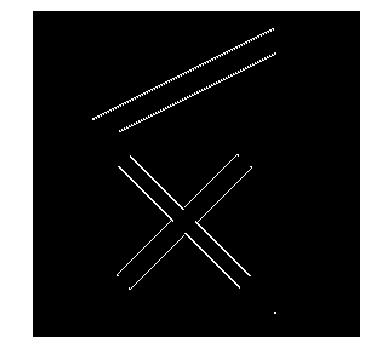
\includegraphics[width=1.3in]{6DL/figures/xu-0401/line-detection-135.png}
	}
	\caption{~~A 135 degree line detection done with convolutions.}
	\label{line:detect8}
\end{figure}

%\begin{figure}[H]
%	\centering
%	\subfigure[image]{
%		%\label{fig:subfig:a} %% label for first subfigure
%		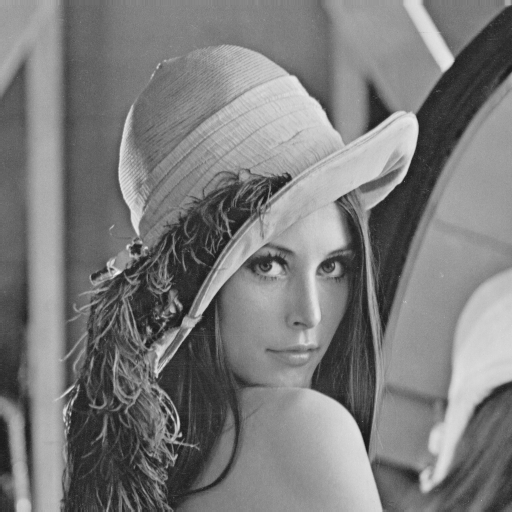
\includegraphics[width=1.3in]{6DL/figures/xu-0401/lena.png}
%	}
%	%\subfigure[filter]{
%%		%\label{fig:subfig:b} %% label for second subfigure
%%		\includegraphics[width=1.0in]{xu-0401/line-detection-135-k.png}
%	%}
%	\subfigure[result]{
%		%\label{fig:subfig:b} %% label for second subfigure
%		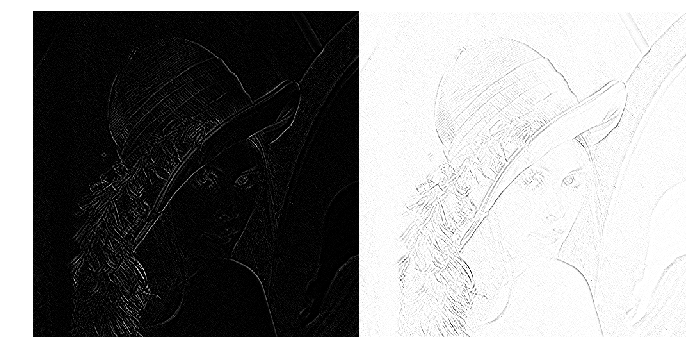
\includegraphics[width=2.6in]{6DL/figures/xu-0401/lena_line_135.png}
%	}
%	\caption{~~A 135 degree line detection done with convolutions.} 
%	\label{line:detect9}
%	%\label{fig:subfig} %% label for entire figure
%\end{figure}


\subsection{Edge detection by 2D Laplacian operator}
The laplacian is the second derivative of the image. It is extremely sensitive to noise, so it isn't used as much as other operators. Unless, of course you have specific requirements.
\begin{figure}[!htbp]
	\centering
	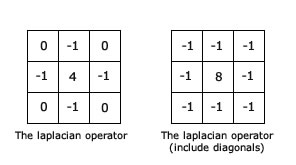
\includegraphics[width=.5\textwidth]{6DL/figures/conv-laplacian.jpg}\\
\end{figure}

Here's the result of the convolution kernel without diagonals:
\begin{figure}[H]
	\centering
	\subfigure[image]{
		%\label{fig:subfig:a} %% label for first subfigure
		
\includegraphics[width=1.3in]{6DL/figures/xu-0401/image.png}
	}
	\subfigure[filter]{
		%\label{fig:subfig:b} %% label for second subfigure
		\includegraphics[width=1.0in]{6DL/figures/xu-0401/laplace-k.png}
	}
	\subfigure[result]{
		%\label{fig:subfig:b} %% label for second subfigure
		
\includegraphics[width=1.3in]{6DL/figures/xu-0401/laplace.png}
	}
	%\label{fig:subfig} %% label for entire figure
\end{figure}
\begin{figure}[H]
	\centering
	\subfigure[image]{
		%\label{fig:subfig:a} %% label for first subfigure
		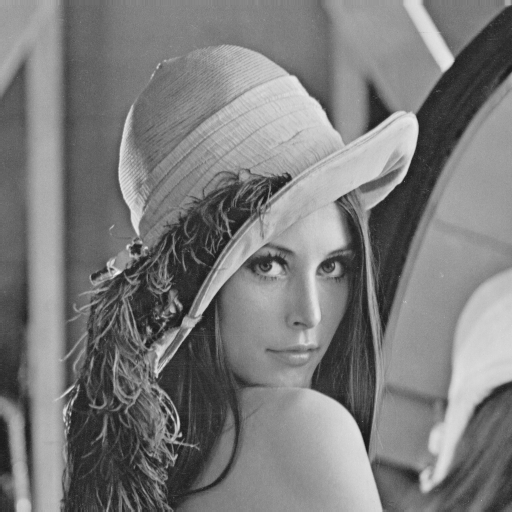
\includegraphics[width=1.3in]{6DL/figures/xu-0401/lena.png}
	}
	%	\subfigure[filter]{
	%		%\label{fig:subfig:b} %% label for second subfigure
	%		\includegraphics[width=1.0in]{xu-0401/laplace-k.png}
	%	}
	\subfigure[result]{
		%\label{fig:subfig:b} %% label for second subfigure
		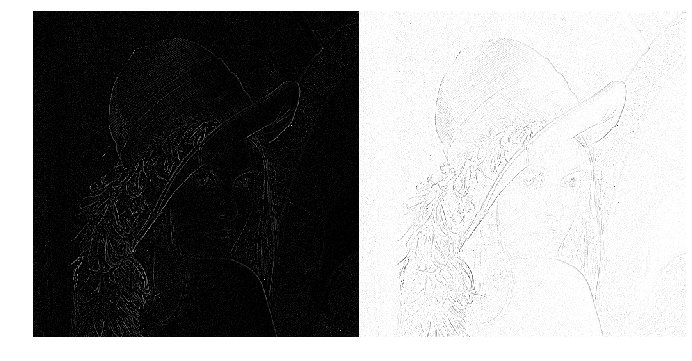
\includegraphics[width=2.6in]{6DL/figures/xu-0401/lena_laplace.png}
	}
	\caption{~~A laplace operator done with convolutions}
	%\label{fig:subfig} %% label for entire figure
\end{figure}

Below is the result of the convolution kernel with diagonals.
\begin{figure}[H]
	\centering
	\subfigure[image]{
		%\label{fig:subfig:a} %% label for first subfigure
		
\includegraphics[width=1.0in]{6DL/figures/xu-0401/image.png}
	}
	\subfigure[filter]{
		%\label{fig:subfig:b} %% label for second subfigure
		\includegraphics[width=1.0in]{6DL/figures/xu-0401/laplace-diag-k.png}
	}
	\subfigure[result]{
		%\label{fig:subfig:b} %% label for second subfigure
		
\includegraphics[width=1.0in]{6DL/figures/xu-0401/laplace-diag.png}
	}
	%\label{fig:subfig} %% label for entire figure
\end{figure}
\begin{figure}[H]
	\centering
	\subfigure[image]{
		%\label{fig:subfig:a} %% label for first subfigure
		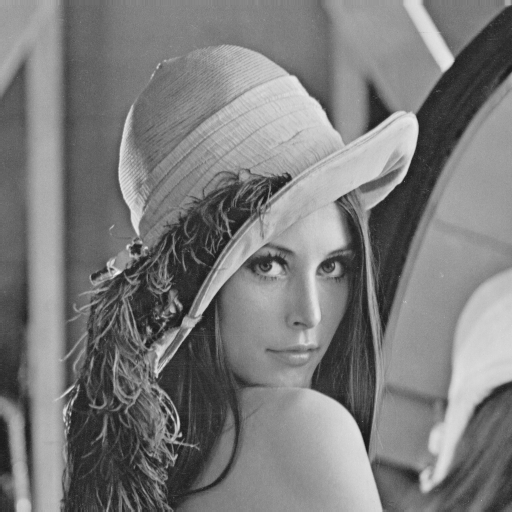
\includegraphics[width=1.3in]{6DL/figures/xu-0401/lena.png}
	}
	%	\subfigure[filter]{
	%		%\label{fig:subfig:b} %% label for second subfigure
	%		\includegraphics[width=1.0in]{xu-0401/laplace-diag-k.png}
	%	}
	\subfigure[result]{
		%\label{fig:subfig:b} %% label for second subfigure
		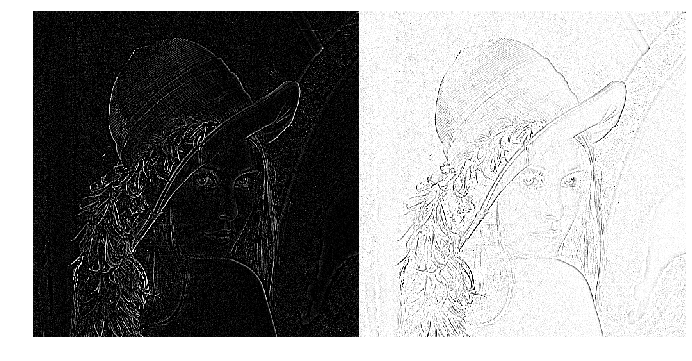
\includegraphics[width=2.6in]{6DL/figures/xu-0401/lena_laplace_diag.png}
	}
	\caption{~~A laplace operator including diagonals are done with convolutions}
	%\label{fig:subfig} %% label for entire figure
\end{figure}

\subsection{The Laplacian of Gaussian}
The laplacian alone has the disadvantage of being extremely sensitive to noise. So, smoothing the image before a laplacian improves the results we get. This is done with a 5x5 image convolution kernel.
\begin{table}[!htbp]
	\centering
	\begin{tabular}{|l|l|l|l|l|}
		\hline
		0  & 0  & -1 & 0  & 0  \\ \hline
		0  & -1 & -2 & -1 & 0  \\ \hline
		-1 & -2 & 16 & -2 & -1 \\ \hline
		0  & -1 & -2 & -1 & 0  \\ \hline
		0  & 0  & -1 & 0  & 0  \\ \hline
	\end{tabular}
\end{table}

Below is the result by applying this image convolution.
\begin{figure}[H]
	\centering
	\subfigure[image]{
		%\label{fig:subfig:a} %% label for first subfigure
		
\includegraphics[width=1.3in]{6DL/figures/xu-0401/image.png}
	}
	\subfigure[filter]{
		%\label{fig:subfig:b} %% label for second subfigure
		\includegraphics[width=1.0in]{6DL/figures/xu-0401/Laplacian-of-Gaussian-k.png}
	}
	\subfigure[result]{
		%\label{fig:subfig:b} %% label for second subfigure
		
\includegraphics[width=1.3in]{6DL/figures/xu-0401/Laplacian-of-Gaussian.png}
	}
	%\label{fig:subfig} %% label for entire figure
\end{figure}

\begin{figure}[H]
	\centering
	\subfigure[image]{
		%\label{fig:subfig:a} %% label for first subfigure
		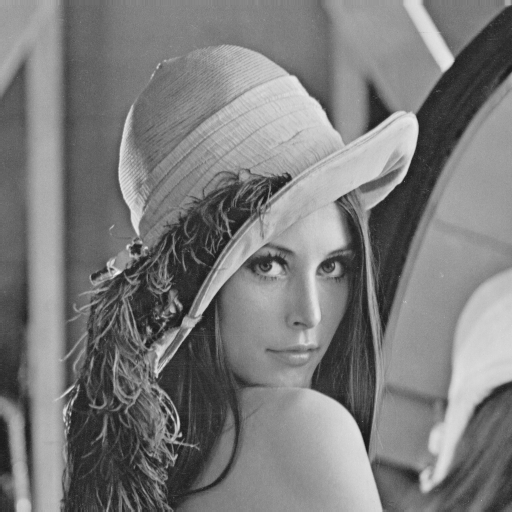
\includegraphics[width=1.3in]{6DL/figures/xu-0401/lena.png}
	}
	%	\subfigure[filter]{
	%		%\label{fig:subfig:b} %% label for second subfigure
	%		\includegraphics[width=1.0in]{xu-0401/Laplacian-of-Gaussian-k.png}
	%	}
	\subfigure[result]{
		%\label{fig:subfig:b} %% label for second subfigure
		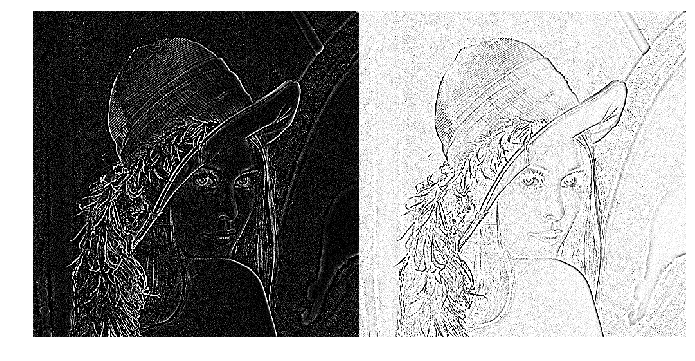
\includegraphics[width=2.6in]{6DL/figures/xu-0401/lena_laplace_gaussian.png}
	}
	\caption{~~A Laplacian of Gaussian operator done with convolutions}
	%\label{fig:subfig} %% label for entire figure
\end{figure}

\subsection{Other examples with ReLU activation}
\begin{figure}[H]
	\centering
	\subfigure[input image]{
		%\label{fig:subfig:a} %% label for first subfigure
		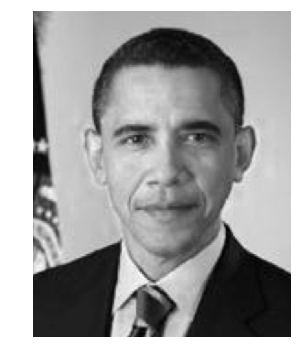
\includegraphics[width=.25\textwidth]{6DL/figures/xu-0401/obama.png}
	}
	\quad 
	\subfigure[filter]{
		%\label{fig:subfig:b} %% label for second subfigure
		\includegraphics[width=.25\textwidth]{6DL/figures/xu-0401/Laplacian-of-Gaussian-k.png}
	}
	\quad
	\subfigure[convolution result]{
		%\label{fig:subfig:b} %% label for second subfigure
		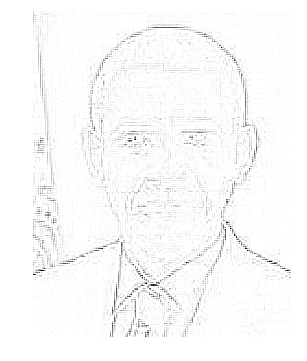
\includegraphics[width=.25\textwidth]{6DL/figures/xu-0401/o_conv.png}
	}
	\\
	\subfigure[result after ReLU]{
		%\label{fig:subfig:b} %% label for second subfigure
		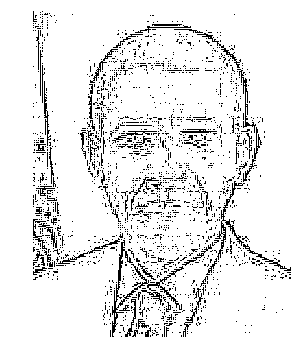
\includegraphics[width=.25\textwidth]{6DL/figures/xu-0401/o_relu.png}
	}
	\quad
	\subfigure[filter]{
		%\label{fig:subfig:b} %% label for second subfigure
		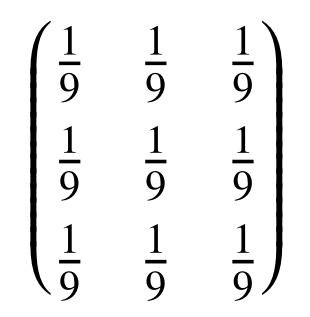
\includegraphics[width=.25\textwidth]{6DL/figures/xu-0401/blur--.png}
	}
	\quad
	\subfigure[result after average]{
		%\label{fig:subfig:b} %% label for second subfigure
		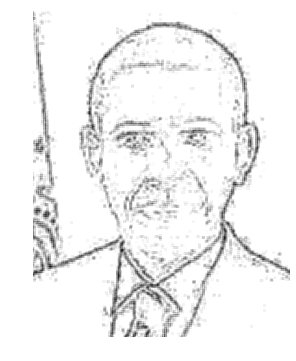
\includegraphics[width=.25\textwidth]{6DL/figures/xu-0401/o_avg.png}
	}
	%\caption{~~A Laplacian of Gaussian operator done with convolutions}
	%\label{fig:subfig} %% label for entire figure
\end{figure}

%\begin{figure}[H]
%	\centering
%	\subfigure[image]{
%		%\label{fig:subfig:a} %% label for first subfigure
%		\includegraphics[width=.25\textwidth]{6DL/figures/xu-0401/trump.png}
%	}
%	\quad 
%	\subfigure[filter]{
%		%\label{fig:subfig:b} %% label for second subfigure
%		\includegraphics[width=.25\textwidth]{6DL/figures/xu-0401/Laplacian-of-Gaussian-k.png}
%	}
%	\quad
%	\subfigure[filter]{
%		%\label{fig:subfig:b} %% label for second subfigure
%		\includegraphics[width=.25\textwidth]{6DL/figures/xu-0401/t_conv.png}
%	}\\
%	\subfigure[ReLU]{
%		%\label{fig:subfig:b} %% label for second subfigure
%		\includegraphics[width=.25\textwidth]{6DL/figures/xu-0401/t_relu.png}
%	}
%	\quad
%	\subfigure[filter]{
%		%\label{fig:subfig:b} %% label for second subfigure
%		\includegraphics[width=.25\textwidth]{6DL/figures/xu-0401/blur--.png}
%	}
%	\quad
%	\subfigure[average]{
%		%\label{fig:subfig:b} %% label for second subfigure
%		\includegraphics[width=.25\textwidth]{6DL/figures/xu-0401/t_avg.png}
%	}
%	%\caption{~~A Laplacian of Gaussian operator done with convolutions}
%	%\label{fig:subfig} %% label for entire figure
%\end{figure}


\iffalse
\subsection{Some other examples}

\subsubsection{Edge detection}
The above kernels are in a way edge detectors. Only difference between the kernels is that they have separate components for horizontal and vertical lines. A way to "combine" the results is to merge the convolution kernels. The new image convolution kernel looks like this:
\begin{table}[!htbp]
	\centering
	\begin{tabular}{|l|l|l|}
		\hline
		-1 & -1 & -1 \\ \hline
		-1 & 8  & -1 \\ \hline
		-1 & -1 & -1 \\ \hline
	\end{tabular}
\end{table}

Below result I got with edge detection:

\begin{figure}[H]
	\centering
	\subfigure[image]{
		%\label{fig:subfig:a} %% label for first subfigure
		\includegraphics[width=1.3in]{6DL/figures/xu-0401/image.png}
	}
	\subfigure[filter]{
		%\label{fig:subfig:b} %% label for second subfigure
		\includegraphics[width=1.0in]{6DL/figures/xu-0401/edge-detection-k.png}
	}
	\subfigure[result]{
		%\label{fig:subfig:b} %% label for second subfigure
		\includegraphics[width=1.3in]{6DL/figures/xu-0401/edge-detection.png}
	}
	%\label{fig:subfig} %% label for entire figure
\end{figure}

\begin{figure}[H]
	\centering
	\subfigure[image]{
		%\label{fig:subfig:a} %% label for first subfigure
		\includegraphics[width=1.3in]{6DL/figures/xu-0401/lena.png}
	}
%	\subfigure[filter]{
%		%\label{fig:subfig:b} %% label for second subfigure
%		\includegraphics[width=1.0in]{xu-0401/edge-detection-k.png}
	%}
	\subfigure[result]{
		%\label{fig:subfig:b} %% label for second subfigure
		\includegraphics[width=2.6in]{6DL/figures/xu-0401/lena_edge_detection.png}
	}
	\caption{~~A edge detection done with convolutions}
	%\label{fig:subfig} %% label for entire figure
\end{figure}


\subsubsection{The Sobel Edge Operator}
The above operators are very prone to noise. The Sobel edge operators have a smoothing effect, so they're less affected to noise. Again, there's a horizontal component and a vertical component.
\begin{figure}[!htbp]
	\centering
	\includegraphics[width=.4\textwidth]{6DL/figures/sobel}\\
\end{figure}

On applying horizontal component in image , the result was:\\

\begin{figure}[H]
	\centering
	\subfigure[image]{
		%\label{fig:subfig:a} %% label for first subfigure
		\includegraphics[width=1.3in]{6DL/figures/xu-0401/image.png}
	}
	\subfigure[filter]{
		%\label{fig:subfig:b} %% label for second subfigure
		\includegraphics[width=1.0in]{6DL/figures/xu-0401/sobel-detection-0-k.png}
	}
	\subfigure[result]{
		%\label{fig:subfig:b} %% label for second subfigure
		\includegraphics[width=1.3in]{6DL/figures/xu-0401/sobel-detection-0.png}
	}
	%\label{fig:subfig} %% label for entire figure
\end{figure}

\begin{figure}[H]
	\centering
	\subfigure[image]{
		%\label{fig:subfig:a} %% label for first subfigure
		\includegraphics[width=1.3in]{6DL/figures/xu-0401/lena.png}
	}
%	\subfigure[filter]{
%		%\label{fig:subfig:b} %% label for second subfigure
%		\includegraphics[width=1.0in]{xu-0401/sobel-detection-0-k.png}
	%}
	\subfigure[result]{
		%\label{fig:subfig:b} %% label for second subfigure
		\includegraphics[width=2.6in]{6DL/figures/xu-0401/lena_sobel_0.png}
	}
	\caption{~~A horizontal sobel edge operator done with convolutions}
	%\label{fig:subfig} %% label for entire figure
\end{figure}

On applying vertical component in image , the result was:
\begin{figure}[H]
	\centering
	\subfigure[image]{
		%\label{fig:subfig:a} %% label for first subfigure
		\includegraphics[width=1.3in]{6DL/figures/xu-0401/image.png}
	}
	\subfigure[filter]{
		%\label{fig:subfig:b} %% label for second subfigure
		\includegraphics[width=1.0in]{6DL/figures/xu-0401/sobel-detection-90-k.png}
	}
	\subfigure[result]{
		%\label{fig:subfig:b} %% label for second subfigure
		\includegraphics[width=1.3in]{6DL/figures/xu-0401/sobel-detection-90.png}
	}
	%\label{fig:subfig} %% label for entire figure
\end{figure}

\begin{figure}[H]
	\centering
	\subfigure[image]{
		%\label{fig:subfig:a} %% label for first subfigure
		\includegraphics[width=1.3in]{6DL/figures/xu-0401/lena.png}
	}
%	\subfigure[filter]{
%		%\label{fig:subfig:b} %% label for second subfigure
%		\includegraphics[width=1.0in]{xu-0401/sobel-detection-90-k.png}
	%}
	\subfigure[result]{
		%\label{fig:subfig:b} %% label for second subfigure
		\includegraphics[width=2.6in]{6DL/figures/xu-0401/lena_sobel_90.png}
	}
	\caption{~~A vertical sobel edge operator done with convolutions}
	%\label{fig:subfig} %% label for entire figure
\end{figure}







\subsubsection{Simple box blur}\footnote{The following examples are from the website, http://aishack.in/tutorials/image-convolution-examples/ }
Here's a first and simplest example. This convolution kernel has an averaging effect. So you end up with a slight blur. The image convolution kernel is:
\begin{table}[!htbp]
	\centering
	\begin{tabular}{|l|l|l|}
		\hline
		1/9 & 1/9 & 1/9 \\ \hline
		1/9 & 1/9 & 1/9 \\ \hline
		1/9 & 1/9 & 1/9 \\ \hline
	\end{tabular}
\end{table}

Note that the sum of all elements of this matrix is 1.0. This is important. If the sum is not exactly one, the resultant image will be brighter or darker.

Here's a blur that I got on an image:

\begin{figure}[H]
	\centering
	\subfigure[image]{
		%\label{fig:subfig:a} %% label for first subfigure
		\includegraphics[width=1.3in]{6DL/figures/xu-0401/image.png}
	}
	\subfigure[filter]{
		%\label{fig:subfig:b} %% label for second subfigure
		\includegraphics[width=1.0in]{6DL/figures/xu-0401/blur--.png}
	}
	\subfigure[result]{
		%\label{fig:subfig:b} %% label for second subfigure
		\includegraphics[width=1.3in]{6DL/figures/xu-0401/blur.png}
	}
	%\label{fig:subfig} %% label for entire figure
\end{figure}

\begin{figure}[H]
	\centering
	\subfigure[image]{
		%\label{fig:subfig:a} %% label for first subfigure
		\includegraphics[width=1.3in]{6DL/figures/xu-0401/lena.png}
	}
	\subfigure[filter]{
		%\label{fig:subfig:b} %% label for second subfigure
		\includegraphics[width=1.0in]{6DL/figures/xu-0401/blur--.png}
	}
	\subfigure[result]{
		%\label{fig:subfig:b} %% label for second subfigure
		\includegraphics[width=1.3in]{6DL/figures/xu-0401/lena_blur.png}
	}
	\caption{~~A simple blur done with convolutions}
	%\label{fig:subfig} %% label for entire figure
\end{figure}

\subsubsection{Gaussian blur}
Gaussian blur has certain mathematical properties that makes it important for computer vision. And you can approximate it with an image convolution. The image convolution kernel for a Gaussian blur is in Table \ref{Gaussianblur}. The result in shown in Figure \ref{lena:Gaussian}.
\begin{table}[!ht]
	\centering
	\begin{tabular}{|l|l|l|l|l|l|l|}
		\hline
		0 & 0  & 0   & 5   & 0   & 0  & 0 \\ \hline
		0 & 5  & 18  & 32  & 18  & 5  & 0 \\ \hline
		0 & 18 & 64  & 100 & 64  & 18 & 0 \\ \hline
		5 & 32 & 100 & 100 & 100 & 32 & 5 \\ \hline
		0 & 18 & 64  & 100 & 64  & 18 & 0 \\ \hline
		0 & 5  & 18  & 32  & 18  & 5  & 0 \\ \hline
		0 & 0  & 0   & 5   & 0   & 0  & 0 \\ \hline
	\end{tabular}
	\caption{The image convolution kernel for a Gaussian blur.}
	\label{Gaussianblur}
\end{table}
\begin{figure}[H]
	\centering
	\subfigure[image]{
		%\label{fig:subfig:a} %% label for first subfigure
		\includegraphics[width=1.3in]{6DL/figures/xu-0401/image.png}
	}
	\subfigure[filter]{
		%\label{fig:subfig:b} %% label for second subfigure
		\includegraphics[width=1.0in]{6DL/figures/xu-0401/g-blut-k.png}
	}
	\subfigure[result]{
		%\label{fig:subfig:b} %% label for second subfigure
		\includegraphics[width=1.3in]{6DL/figures/xu-0401/Gaussian-blur.png}
	}
	%\caption{A Gaussian blur done with convolutions}
\end{figure}

\begin{figure}[H]
	\centering
	\subfigure[image]{
		%\label{fig:subfig:a} %% label for first subfigure
		\includegraphics[width=1.3in]{6DL/figures/xu-0401/lena.png}
	}
	\subfigure[filter]{
		%\label{fig:subfig:b} %% label for second subfigure
		\includegraphics[width=1.0in]{6DL/figures/xu-0401/g-blut-k.png}
	}
	\subfigure[result]{
		%\label{fig:subfig:b} %% label for second subfigure
		\includegraphics[width=1.3in]{6DL/figures/xu-0401/lena_G_blur.png}
	}
	\caption{~~A Gaussian blur done with convolutions}
	\label{lena:Gaussian}
\end{figure}

\fi

\subsection{Summary}
These examples show  how different convolution kernels modify an image in different ways. Note that the filter plays an important role in detecting edges on an image.
